%-----------------------------------------------------------------------------------------------------------
% Everything before \begin{document} and
% \end{document} is called Preamble. The Preamble
% sets up your document. The preamble typically specifies
%   the document class
%   languages
%   imports packages by using \usepackage{package_name} command
%-----------------------------------------------------------------------------------------------------------

%-----------------------------------------------------------------------------------------------------------
% Note: A latex command consist of a backslash, command name, argument (with {}) #
% and optional arguments (with []), e.g.
% \command_name[optonal_argument1, optional_argument2 ..]{arugment}
%-----------------------------------------------------------------------------------------------------------

%-----------------------------------------------------------------------------------------------------------
% \documentclass have to be the first command of each latex file and 
% defines layout and class of the document.
%   [options]: contains options to define the layout of the document (fontsize, paper, columns ...) 
%   {class}: defines the class of the document. Possible classes are:
%               - article: for scientifc journals
%               - book: for books
%               - reports: for longer reports with several chapters, thesis, small books
%               - letter: for letters
%               - slides: for slides
%               - beamer: for latex presentations
%   Sources: 
%       https://texblog.org/2013/02/13/latex-documentclass-options-illustrated/ (for options)
%       https://en.wikibooks.org/wiki/LaTeX/Document_Structure#Document_classes (for classes)
%-----------------------------------------------------------------------------------------------------------
\documentclass[a4paper,11pt,onecolumn]{report}


%-----------------------------------------------------------------------------------------------------------
% The \usepackage{package_name} commands imports external packages (here: graphicx)
% to provide latex with external features.
%-----------------------------------------------------------------------------------------------------------
% graphicx package contains commands and features to import external graphic file, i.e.
%   - \includegraphics{picture_name} command to import graphics.
%   - \graphicspath{{path/to/your/images/}} command to tell latex where the graphics are located
\usepackage{graphicx}
\graphicspath{{images}}

\usepackage{array} % to use m and b flags for the table columns
% package needed for tabularx enviornment
\usepackage{tabularx}
% package needed for \mutlirow command
\usepackage{multirow}
\usepackage{longtable}

% package needed to apply colours to table rows
% option table specifies that package is only applied to table environment
\usepackage[table,dvipsnames]{xcolor}

% options to load named color with the color package 
% \usepackage[usenames, dvipsnames]{color}

% defintion of your own colors
% The \definecolor{<defined_color_name>}{<model>}{values...} let you 
% define your own colors. After the definition of you own colors you can
% easily use them by the \color{<defined_color_name>} command within the document

% the following command defines a color with the rgb model (red, green, blue) 
% with comma seperated values from 0-1 for each color. 
\definecolor{MyColor1}{rgb}{0.8,0.2,0.3}
% the following command defines a color with the RGB model (red, green, blue)
% with integer values from 0-255 for each color
\definecolor{MyColor2}{RGB}{255,0,0}
% the following command defines a color with the HTML model means with a
% Hexadecimal code
\definecolor{MyColor3}{HTML}{AA1202}    
% the following command defines a color by its grey scale, i.e. the specified 
% color a mixed with gray.
\definecolor{MyColor4}{gray}{0.5}
% After the definition of your colors you can easily use theme with the \color 
% command with it's defined names, e.g. \color{MyColor1}

% Alternative you can mix colors with the \colorlet command, \usepackage{xcolor} 
% required. 
% The following command defines a color with 70% RubineRed and 30% white
\colorlet{MyColor6}{RubineRed!70}
% The following command defines a color with 10% green and 90% orange
\colorlet{MyColor5}{green!10!orange}


% to define the layout of the page (such aus width, length,
% margins, etc.) use the \usepackage{geometry} command
% the following command creates a document with a text area
% with 6 inches wide and 8 inches height
%\usepackage[a4paper,total={6in,8in}]{geometry}

% You can seperate the options from the geometry package by using 
% the geometry package
\usepackage{geometry}
% following command creates a4paper with a textarea 6in wide and 8in height
% \geometry{a4paper, total={6in,8in}}
% following command creates legalpaper in portrait mode and with 2in margin 
% \geometry{legalpaper, portrait, margin=2in}


% layout package includes commands to visualize documents layout
\usepackage{layout}

% package lipsum includes command(s) to create dummy text
\usepackage{lipsum}
% package blindtext includes command(s) to create dummy text
\usepackage{blindtext}

% package hyperref to add hyper links to the document for the references etc.
\usepackage{hyperref}
% \hypersetup command will set up the options to configure the behaviour 
% of the links within the document
% https://de.overleaf.com/learn/latex/Hyperlinks#Reference_guide (for all options)
\hypersetup{
    % the hypersetup can have following options:
    % colorlinks defines if links should be coloured or not
    colorlinks=true,    
    % linkcolor defines the color of the links
    linkcolor=green,
    % filecolor defines the color of links to local files
    filecolor=yellow,
    % urlcolor defines the color of links to websites
    urlcolor=blue,
    % defines the title of the pdf
    pdftitle={Example pdf title},
    % defines the appearance mode at the opening of the pdf with a pdf reader.
    pdfpagemode=FullScreen,
}

% 1 import package biblatex required for bibliography
\usepackage{biblatex}
% 2 store your references/citations in a .bib file 
% and import it with the \addbibresource{bibliographic resource} command 
\addbibresource{./references/chatbot.bib}

% package to use the import command
\usepackage{import}

% You can also set the page style in Latex by using the 
% \pagestyle{<style>} and \thispagestyle{<style>} commands
% There are four styles for <style> argument available
% empty: no header, no footer
% plain: no header, footer contains centered pagenumber
% headings: no footer, header contains centered page number and class-specific info
% myheadings: same as headings but it contains user-specific infos instead of class-specific

% usally the for the document defined report contains plain style per default
% The \pagestyle{<style>} commands sets the style for the current and subsequent pages
% \pagestyle{plain}

% The \thispagestyle command sets style only for the current page
% \thispagestyle{plain}

% Import of fancyhdr to set up headers and footers
\usepackage{fancyhdr}

% Import of lastpage package for lastpage command
\usepackage{lastpage}

% This command sets the thickness of the borders of the table to 0.5em
\setlength{\arrayrulewidth}{0.25em}
% This command sets the space between the text and the left/right border of 
% its cell, here to 25pt also other units possible
\setlength{\tabcolsep}{25pt}
% \renewcommand{\arraystretch}{1.5} commands set the height of each row of a table
\renewcommand{\arraystretch}{1.5}

% Import package amsmath for \newtheorem command
\usepackage{amsmath}

%-----------------------------------------------------------------------------------------------------------
% For adding a title, author and date, latex need to include first the following three commands
% in preamble. In a second you have to include the \maketitle command between \begin{docuemtn} and
% \end{document}
%-----------------------------------------------------------------------------------------------------------
% adds a title
\title{Soccer is great \& Politics sucks!}   
% adds a author with footnote to thank, e.g. your institution or coworker
\author{Sefa Kutlu!\thanks{Thanks to Albert Einstein whose shared his great knowledge with us. }}
% adds a date (\today for todays date or a apsicifc date, e.g. \date{August 2022})
\date{\today}                           

%-----------------------------------------------------------------------------------------------------------
% The content of a document have to be added between the \begin{document} and \end{document}
%-----------------------------------------------------------------------------------------------------------
\begin{document}

    % The \pagenumbering{<style>} command sets the style of the page number, the style 
    % argument can on of these five:
    % arabic (1,2,3,...)
    % alph (a,b,c,...) 
    % Alph (A,B,C,...)
    % roman (i,ii,iii)
    % Roman (I,II,III)
    \pagenumbering{arabic}   % sets the page numbering style to uppercase Roman style

    % \maketitle commands adds the information defined above with title, author date commands to the document
    % have to be the first command within \begin{document} and \end{document}
    \maketitle
    Hello Latex!. This is an example sentence written by me.
    % \\ new line without new paragraph command
    \\
    % bold, italic, underline commands
    % \textbf{word}: The word in braces will displayed bold
    The last word should be \textbf{bold}.      
    \\
    % \textit{word}: The word in braces will displayed italic
    The last word should be \textit{italic}.
    \\
    % \underline{word}: The word will be underlined
    The last word should be \underline{underlined}.
    \\
    % combine of the three commands from above
    The last three words should be \textbf{\textit{\underline{bold italic underlined}}}.
    \\
    % \emph{argument} effect on its argument will depends on the context, i.e.
    % the emphasized text italicized, but behaviour is reversed inside italic text
    This sentence contains an \emph{emphasized word}, but the rest of the text remains normal.
    \\
    \textit{This italic sentence contains a not italic \emph{word}}
    \\
    % \emph{argument} inside a bold sentence the emphasized word is displayed italic
    \textbf{This bold sentence contains an emphasized \emph{word}}.
    \\

    % It isn't compelling to wrap the \includegraphics{your_file} between
    % \begin{figure} and \end{figure}, but advisable to add a label and caption 
    % to the graphic.
    \begin{figure}
        % \centering command centers the graphic.
        \centering
        % \includegraphics loads the image besiktas_team
        % \textwidth command returns the width of a text on a page
        % [width=\textwidth] option adjusts the width of graphic to the textwidth
        % instead of using \textwidth you can specifiy a specific width with cm, inch ..., e.g.
        % width=2.3cm
        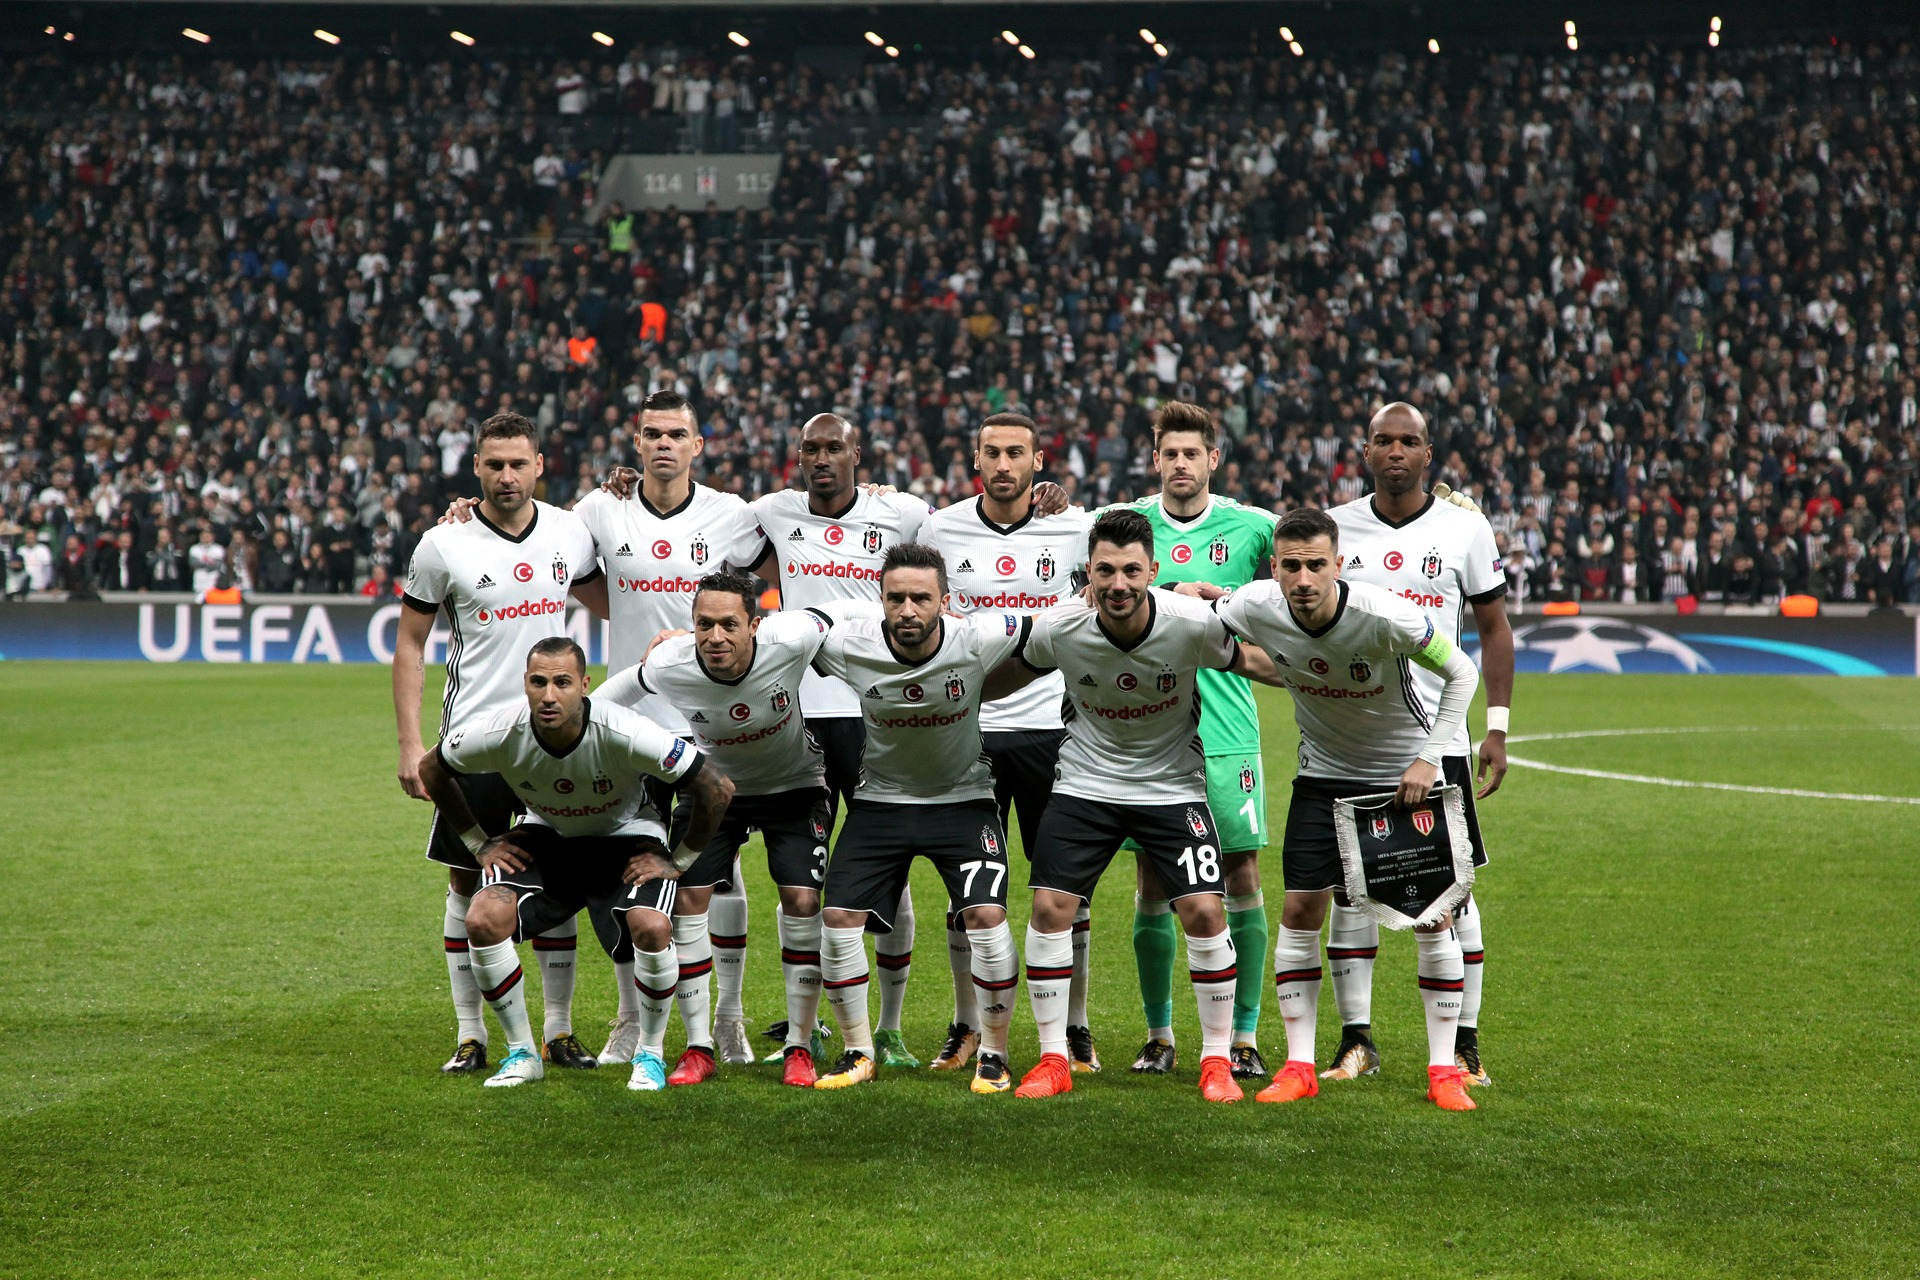
\includegraphics[width=0.75\textwidth]{besiktas_team} % sets width to 75% of textwidth
        % \caption{arg} command gives the figure a caption
        \caption{Besiktas JK 2017/2018}
        % \label{fig:<name>} command labels the figure and generates a number to reference the image within the document
        % with \ref{fig:<name>}
        % \label command have to be the last in a figure, otherwise the reference won't displayed.
        \label{fig:besiktas_team}     
    \end{figure}

    % This \includegraphics command can contain following options, comment or comment out the options you want
    % to try out.
    \begin{figure}
        \centering
        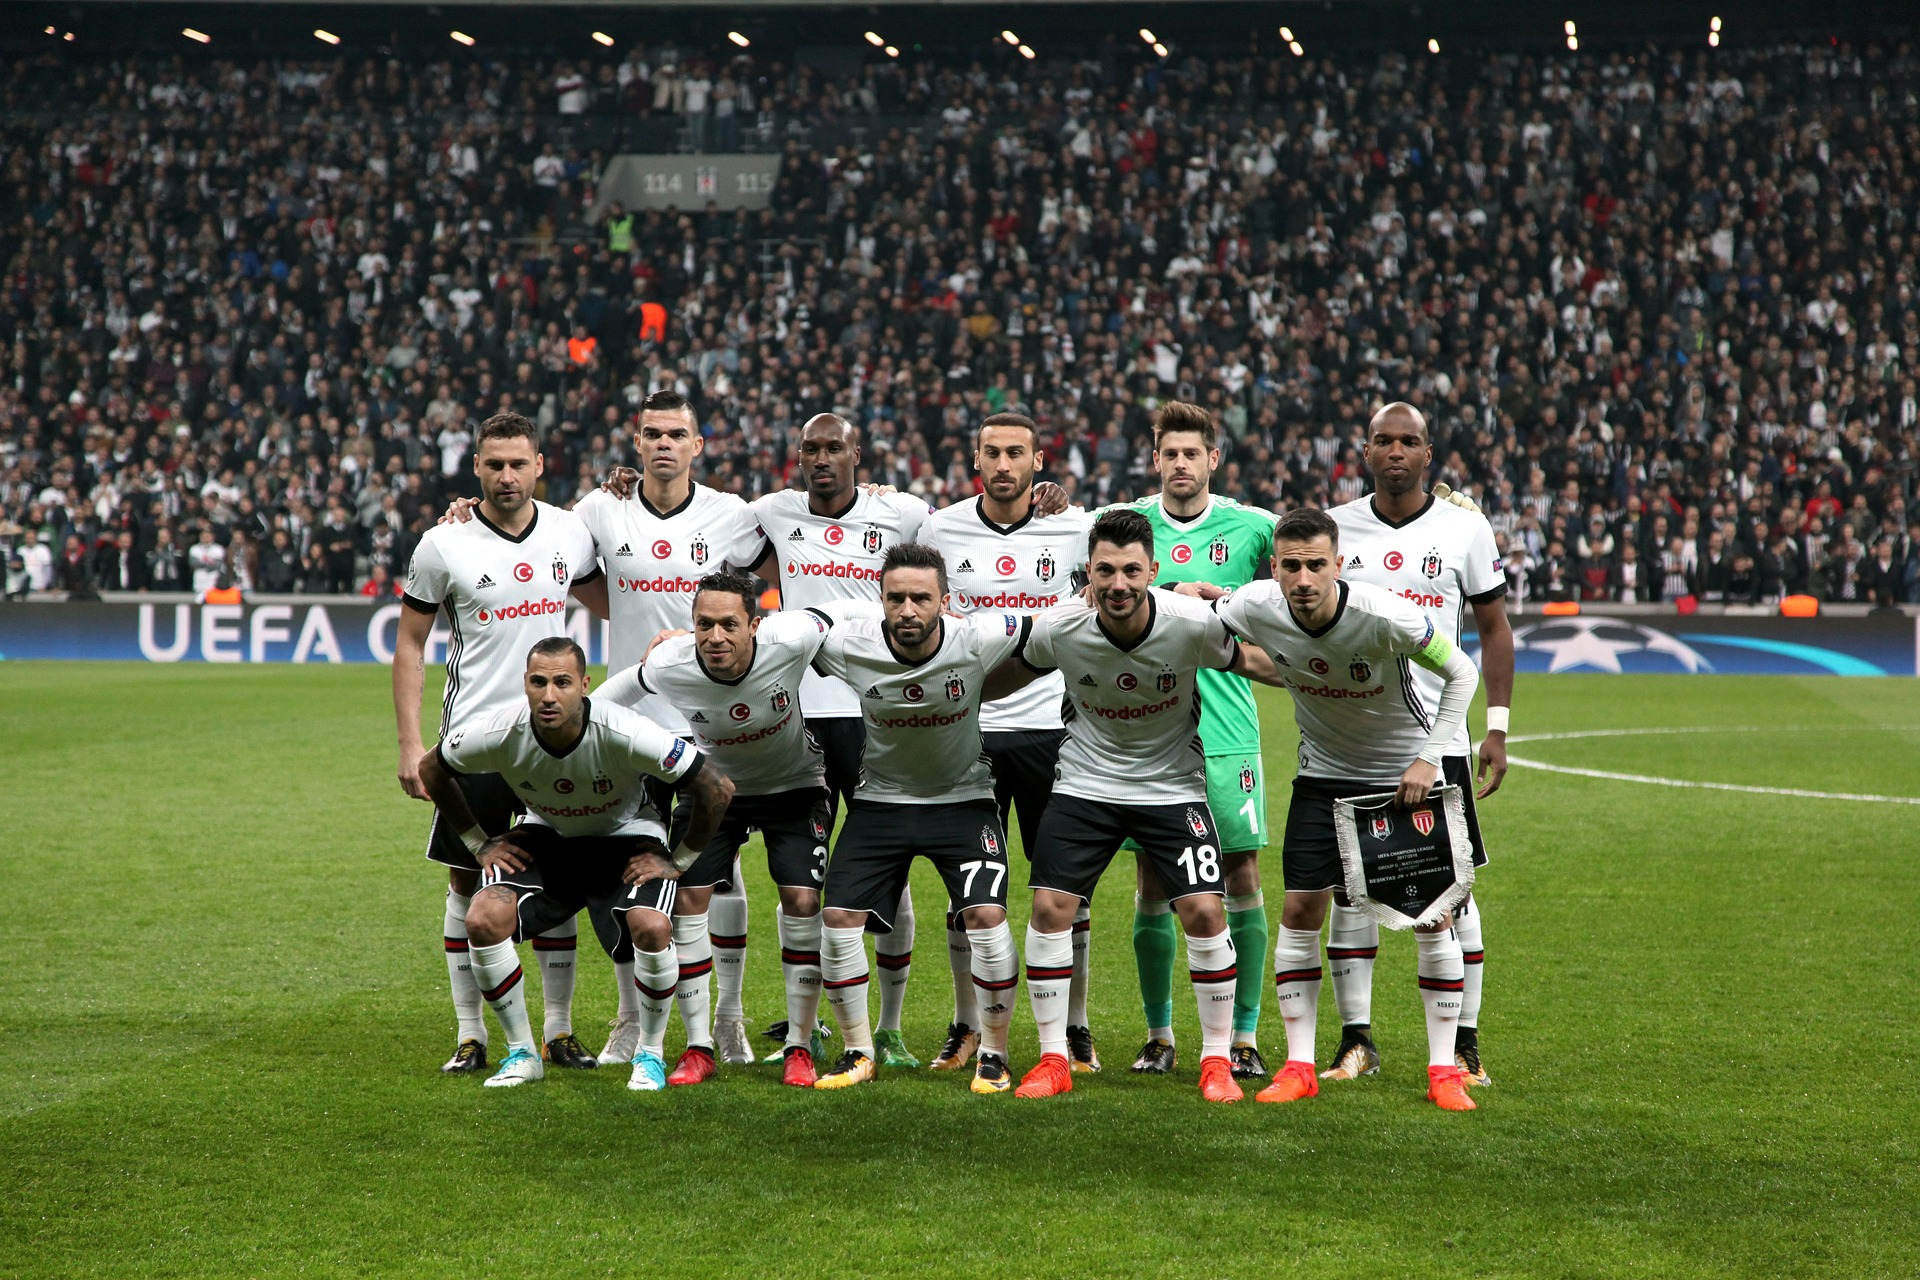
\includegraphics
        [%scale=0.10,% scale scales graphic based on specified scale factor
         %width=5.5cm,% width scales graphic based on specified width 
         height=3.5cm,% height scales graphic based on specified height
         %draft % is draft set, latex displays a placeholder (path of file) instead of loading the image. Accelerates the translation process of document.
         angle=-90,% angle rotate the graphic based on specified value, positiv values = counterclockwise, negative values = clockwise,
         % -90 rotates the graphics 90 degree clockwise
        ]{besiktas_team}
        \caption{height 3.5cm and rotate -90 degree (clockwise)}
        \label{fig:besiktas_team_with_several_options}
    \end{figure}

    % \ref{figure} command is substituted by the number corresponding to the referenced figure 
    % \pageref{figure} command is substituted by the page number on which the figure is displayed.  
    The Figure \ref{fig:besiktas_team} is on page \pageref{fig:besiktas_team}.

    \clearpage

    %----------------------
    %   Lists
    %----------------------
    % An unordered list is created with the enviroment \begin{itemize} ... \end{itemize}
    % and items are defined inside them with: \item example item 
    % for example:
    \begin{itemize}
        \item an item
        \item another item
        \item useless item
    \end{itemize}
    
    % An ordered list is created with the enviroment \begin{enumerate} ... \end{enumerate}
    % and items are defined inside them with: \item example item 
    % for example:
    \begin{enumerate}
        \item first item
        \item second item
        \item third item
    \end{enumerate}

    %----------------------
    %   Math
    %----------------------
    % A Huge advantage of Latex is the ease of writing mathematical expressions.
    % There are two modes to write mathematical expression:
    % 1. inline math mode: used to write formulas that are part of a paragraph
    % 2. display math mode: used to write formulas that are not part of text or paragraphs
    % and are set on separate lines.

    % Inline math mode
    % To typeset inline math mode u can use one of the these delimiter pairs:
    % \(...\)
    % $...$
    % \begin{math}...\end{math}
    The following commands demonstrate how you can typeset inline-mode math.\\
    % \textbackslash command creates a \ within text, it can't be used as \ in a text, since 
    % it is a special character reserved for latex commands.
    % Special characters reserved by latex can be used in text with \ before the character
    % e.g. \{ = { (in text), \] = ] (in text).
    With \textbackslash begin\{math\} \dots \textbackslash end\{math\}.
    \begin{math}
        E=mc^2
    \end{math}
    \\
    With \$\dots\$
    $E=mc^2$
    \\
    With \textbackslash (\dots\textbackslash)
    \(E=mc^2\)

    % Display math mode
    % To typeset display-mode math u can one of these delimiter pairs:
    % \[...\]
    % \begin{displaymath} ... \end{displaymath}
    % \begin{equation} ... \end{equation}
    The following commands demonstrate how you can typeset display-mode math
    Here comes some text. Let's see if the formulas 
    \[E=mc^2\]
    \begin{displaymath}
        E=mc^2
    \end{displaymath}
    \begin{equation}
        E=mc^2
    \end{equation}
    will appear in this paragraph
    or in a new line.

    % More Complex Math
    % _ for subscripts
    % ^ for Superscripts
    Subscripts (dt. index) in math mode are written as $a_b$ (\$a\_b\$). \\
    Superscripts (dt. exponent) in math mode are written as $a^b$ (\$a\^{}b\$). \\

    % Example for complex math formulas
    % \dots command displays ...
    % Hint: Group subscripts & Superscripts with multiple variables or numbers
    % inside {...}
    \[T^{i_1i_2 \dots i_p}_{j_1,j_2 \dots j_q} = 
    T(x^{i_1},\dots,x^{i_p},e_{j_1},\dots,e_{j_q})\]

    % Integrals are written with the \int command.
    % Append \int ^<char>_
    Integrals are written by using \textbackslash int command. You can
    append, e.g. \^{}5\_1 to define 5 as upper and 1 as 
    lower boundary. Also, possible to append it in the revert order like 
    \_{}1\^{}5. Both will produce the same output. 
    \[\int^5_1\]
    \[\int_1^5\]


    Fractions are written by using \textbackslash frac\{Numerator\}\{Denominator\}, e.g.
    \begin{displaymath}
        \frac{Numerator}{Denominator}
    \end{displaymath}

    The following formula describes using the \textbackslash int and
    \textbackslash frac \{Numerator\}\{Denominator\}
    \begin{equation}
        \int^1_0 \frac{dx}{e^x} = \frac{e-1}{e}    
    \end{equation}

    % Example for lower- and uppercase greek letters
    % lowercase leters
    \clearpage
    Example for lowercase Greek letters.
    \begin{itemize}
        \item $\omega$
        \item $\delta$
        \item $\gamma$
        \item ...
    \end{itemize}

    Example for uppercase Greek letters
    \begin{itemize}
        \item $\Omega$
        \item $\Delta$
        \item $\Gamma$
        \item ...
    \end{itemize}
    Greek letters have their own commands (e.g.\textbackslash omega for $\omega$). To produce lowercase Greek
    letters you have to write the corresponding command of the letter in 
    lowercase. For the uppercase Greek letters you have write the first
    letter of the command in uppercase.\\

    % Example for sin, cos and log
    Example for sin, cos and log, Attention: NEVER FORGET TO PUT MATH FORMULAS
    BETWEEN MATH MODE COMMANDS!!!.
    \begin{itemize}
        \item $\sin(\beta)$, latex command:  \$\textbackslash sin(\textbackslash beta)\$ 
        \item $\cos(\alpha)$, latex command:  \$\textbackslash cos(\textbackslash alpha)\$ 
        \item $\log(x)$, latex command:  \$\textbackslash log(x)\$ 
    \end{itemize}

    % Math square root 
    Example for square root. The command: \textbackslash sqrt\{expression\}
    \[\sqrt{x^2+1}\]

    % scientifc articles uses abstracts a brief overview of their core
    % topics or arguments, in latex you can write abstracts between 
    % \begin{abstract} ... \end{abstract}
    \begin{abstract}
        Here is your first abstract without a sense.
    \end{abstract}

    % Paragraph 
    % press enter twice to create a new paragraph
    Hello new paragraph! 
    
    Hello second new paragraph!

    % New lines without new paragraph are created with
    % \\ or \newline command
    % \verb|<command>| command to display latex commands in text/pdf.
    This is a sentence to demonstrate the effect of the \verb|\\.|\\
    This sentence should be on a new line. Bingo it does!
    Also, it is possible to create a new line with \verb|\newline|\newline
    command. Great!, now we know how to create new paragraphs and new lines.

    % chapter, section and subsection
    % \chapter command creates a chapter, only available in book and report
    \chapter{First Chapter} 
    % \section command creates a section
    \section{Introduction}
    This is the Introduction.
    \section{Second Section}
    This is the second Section.
    % \subsection command creates a subsection
    \subsection{First subsection}
    This is the first subsection of the second section.
    % \section* creates an unnumbered section
    \section*{Unnumbered section}
    % unnumbered sections wont be added with the \tableofcontents command
    % you have to add them manually by the following command
    \addcontentsline{toc}{section}{Unnumbered section}
    This is an example for an unnumbered section
    % Note: The commands with (*) asterisk disable the automatic numbering

    % Also possible a parts, paragraphs and subparagraphs
    \part{A new part} % only in book and report
    \paragraph{A new Paragraph}
    This is an example paragraph with some text. The text here has no meaning 
    and serves as placeholder.
    \subparagraph{A new subparagraph}
    This is a subparagraph
    
    %----------------------------
    %   Tables
    %----------------------------
    \section{Table}
    Section for tables in latex
    \newline
    \newline
    This is a simple table with content centered in the middle and 
    no borders
    % Embedd the table in a table enviornment to make it available for
    % list of tables, give it a caption an label!
    \begin{table}[h]    % h = table are placed (exactly) here 
        % center environment to center the table, alternatively use \centering
        \begin{center}
            % \begin{tabular}[pos]{cols} ... \end{tabular} creates a table
            % with the arguments specified in pos and cols.
            % the following table have { c c c } as argument means that 
            % we want a table with tree columns and the content of each column
            % have to be centered
            % instead of c u can also use 
            % r (right-justified content)
            % l (left-justified content)
            \begin{tabular}{ c c c }
                % each columns are separated by &
                % \\ indicates a new row
                cell1 & cell2 & cell3 \\    
                % last row doesn't need \\, if nothing follows
                cell4 & cell5 & cell6 \\    
                cell7 & cell8 & cell9       
            \end{tabular}
            % caption for table
            \caption{Simple table with no borders and content centered}
            % label to reference the table within the document
            \label{table:simple_table}
        \end{center}
    \end{table}

    % A advanced table
    \begin{table}[h]
        \centering  % centers the table
        % the | char creates a border, while || creates a double border
        % m{<width>} creates a column with specified width and 
        % aligns the text in middle, also possible: (requires: \usepackage{array})
        % p{<width>} creates column with specified width and aligns text at top
        % b{<width>} creates column with specified width and aligns text at bottom 
        % (requires: \usepackage{array} 
        % creates 4 columns with left centered right, and paragraph column with 4.2em width middle centered text
        \begin{tabular}{|| l | c | r | m{4.2em} ||}
            \hline  % draw a horizontal line with \hline command to create a 
            % border for the top 
            cell left & cell centered & cell right & paragraph cell with 3.5em width and the content is aligned to the middle \\
            % cline draws partial line between the specified columns
            % Note: left border starts by 1.
            \cline{3-4}
            cell2 left & cell2 centered & cell2 right & paragraph cell2 \\
            % double \hline commands create a gap within the table
            % useful for, e.g. separating table title from table content.
            \hline
            \hline
            cell3 left & cell3 centered & cell3 right & paragraph cell3 \\
            \hline 
        \end{tabular}
        \caption{Table with borders left, right aligned and centered content}
        \label{table:intermediate_table}
    \end{table}

    % for specify the width for entire table and evenly distribute the space within
    % use tabularx environment
    % 1. \usepackage{tabularx}
    \begin{tabularx}{0.8\textwidth} { % uses 80% of the text width
        % the prefix inside braces sets the alignment, i.e.
        % firts column to right, second to center and third to left
        | >{\raggedright\arraybackslash}X
        | >{\centering\arraybackslash}X
        | >{\raggedleft\arraybackslash}X |
    }
    \hline
    item 11 & item 12 & item 13 \\
    \hline
    item 21 & item 22 & item 23 \\
    \hline
    \end{tabularx}


    %-------------------------------------------------------------
    % Multicolumn and multirow
    %-------------------------------------------------------------
    % the \multicolumn command allows you to merge several columns
    % 1. \usepackage{multirow}
    \begin{table}[h]
        \begin{tabular}{ |p{3cm} | p{3cm} | p{3cm} | p{3cm}| }
            \hline
            % the \multicolumn command has 3 arguments
            % {4} stands for the number of columns to be merged
            % {| c |} delimiters and alignment of the colum, centered with vertical
            % line at each side of the cell
            % {This is a merged column} can contain any text to be displayed within
            % the text.
            \multicolumn{4}{|c|}{This is a merged column} \\
            \hline 
            content 1 & content 2 & content 3 & content 4 \\
            content 4 & content 5 & content 6 & content 7 \\
            \hline
    
        \end{tabular}
        \caption{ table with multicolumn command}
        \label{table:table_multicolumn}        
    \end{table}

    % to combine the rows you need to add the \multirow package
    % \usepackage{multirow}
    \begin{table}[h]
        \centering
        \begin{tabular}{|c|c|c|}
            \hline
            \multicolumn{3}{|c|}{multirow table} \\
            \hline
            % the \multirow command takes also 3 arguments
            % {3} defines how many columns should be combined
            % {5em} defines the width of the combined columns
            % {multiple row} contains text to be displayed
            \multirow{3}{5em}{multiple row} & col2 & col3 \\ 
                                            & col4 & col5 \\
                                            & col6 & col7 \\
            \hline
        \end{tabular}
        \caption{This table is using the multirow command}
        \label{table:table_multirow}
    \end{table}

    %---------------------------------------------------------
    % Multipage Tables
    %---------------------------------------------------------

    % If you want to insert very long tables, which take up to one or more pages
    % then use the \longtable command
    % First add \usepackage{longtable} to preamble of your document
    \begin{longtable}[c]{ | c | c | }
        \caption{Long Table}
        \label{table:table_long} \\
        
        % Defintion of the first head of the table
        \hline
        \multicolumn{2}{ | c | }{Begin of table} \\
        \hline
        Something & something else  \\
        \hline
        Extra & Extra2 \\
        \hline
        % Everything above this command will appear at the beginning of the 
        % table on the first page
        \endfirsthead

        % Second head defintion
        \hline
        \multicolumn{2}{ | c | }{Continuation of the table}  \\
        \hline
        Something & something else \\
        \hline
        % Everything between this command and below \endfirshead will appear on 
        % top of table on each page except the first one.
        \endhead

        \hline
        last column & last column \\
        \hline
        % what you put before \endfoot and below \endhead will appear on the end 
        % of each table on each page except the last page
        \endfoot


        \hline
        \multicolumn{2}{ | c | }{End of Table}\\
        \hline
        \hline
        % the elements before this command and \endfoot will be displayed at the 
        % bottom of the table only on the last page.
        \endlastfoot

        % Content of the long table
        Lots of lines & like this\\
        Lots of lines & like this\\
        Lots of lines & like this\\
        Lots of lines & like this\\
        Lots of lines & like this\\
        Lots of lines & like this\\
        Lots of lines & like this\\
        Lots of lines & like this\\
        Lots of lines & like this\\
        Lots of lines & like this\\
        Lots of lines & like this\\
        Lots of lines & like this\\
        Lots of lines & like this\\
        Lots of lines & like this\\
        Lots of lines & like this\\
        Lots of lines & like this\\
        Lots of lines & like this\\
        Lots of lines & like this\\
        Lots of lines & like this\\
        Lots of lines & like this\\
        Lots of lines & like this\\
        Lots of lines & like this\\
        Lots of lines & like this\\
        Lots of lines & like this\\
        Lots of lines & like this\\
        Lots of lines & like this\\
        Lots of lines & like this\\
        Lots of lines & like this\\
        Lots of lines & like this\\
        Lots of lines & like this\\
        Lots of lines & like this\\
        Lots of lines & like this\\
        Lots of lines & like this\\
        Lots of lines & like this\\
        Lots of lines & like this\\
        Lots of lines & like this\\
        Lots of lines & like this\\
        Lots of lines & like this\\
        Lots of lines & like this\\
        Lots of lines & like this\\
        Lots of lines & like this\\
        Lots of lines & like this\\
        Lots of lines & like this\\
        Lots of lines & like this\\
        Lots of lines & like this\\
        Lots of lines & like this\\
        Lots of lines & like this\\
        Lots of lines & like this\\
        Lots of lines & like this\\
        Lots of lines & like this\\
        Lots of lines & like this\\
        Lots of lines & like this\\
        Lots of lines & like this\\
        Lots of lines & like this\\
        Lots of lines & like this\\
        Lots of lines & like this\\
        Lots of lines & like this\\
        Lots of lines & like this\\
        Lots of lines & like this\\
        Lots of lines & like this\\
        Lots of lines & like this\\
        Lots of lines & like this\\
        Lots of lines & like this\\
        Lots of lines & like this\\
        Lots of lines & like this\\
        Lots of lines & like this\\
        Lots of lines & like this\\
        Lots of lines & like this\\
        Lots of lines & like this\\
        Lots of lines & like this\\
        Lots of lines & like this\\
        Lots of lines & like this\\
        Lots of lines & like this\\
        Lots of lines & like this\\
        Lots of lines & like this\\
        Lots of lines & like this\\
        Lots of lines & like this\\
        Lots of lines & like this\\
        Lots of lines & like this\\
        Lots of lines & like this\\
        Lots of lines & like this\\
        Lots of lines & like this\\
        Lots of lines & like this\\
        Lots of lines & like this\\
        Lots of lines & like this\\
        Lots of lines & like this\\
        Lots of lines & like this\\
        Lots of lines & like this\\
        Lots of lines & like this\\
        Lots of lines & like this\\
        Lots of lines & like this\\
        Lots of lines & like this\\
        Lots of lines & like this\\
        Lots of lines & like this\\
        Lots of lines & like this\\
        Lots of lines & like this\\
        Lots of lines & like this\\
        Lots of lines & like this\\
        Lots of lines & like this\\
    \end{longtable}

    %-----------------------------------
    % Table positioning
    %-----------------------------------
    % you can position the table by wraping the tabularx environment
    % in the table enviromnent, like in the following illustration,
    % you can use the following parameters
    % h will place the table here approximately (dt. etwa, ungefähr)
    % t will place the table at the top of the page
    % b will place the table at the bottom of the page
    % p will place the table in a special page. for tables only
    % ! overrides internal latex parameter
    % H places the table at this precise location, like h!
    % h! places the table at this precise location
    % \centering centers the table
    % \[1ex] adds extra space for table
    \begin{table}[]
        \begin{tabular}{ | c | c | c | }
            \hline
                col1 & col2 & col3 \\
                col4 & col5 & col6 \\
            \hline
        \end{tabular}
    \end{table}

    % \listoftables commands adds list of tables with all labeled tables to document
    % it will use the caption of the tables to create the list
    \listoftables

    %---------------------------------------------------------
    %   Change appearance of a table
    %---------------------------------------------------------
    % \setlength{\arrayrulewidth}{length} sets the thickness of the borders of the tables
    % \setlength{\tabcolsep}{length} sets the space between the text and left/right border of its cell
    % \renewcommand{\arraystretch}{1.5} sets the height of each row, here 1.5

    % coloring your cell
    % you can apply colours to the rows of your table by using the xcolor
    % package

    % \rowcolors take 3 arguments
    % {2} specifies the row to start
    % {green!80!yello!50} specifies the color for odd rows
    % {green!80!yellow!40} specifies the color for even rows
    {\rowcolors{2}{green!80!yellow!50}{green!80!yellow!40}
    \centering
    \begin{tabular}{|c|c|}
        \hline
        \multicolumn{2}{|c|}{Table with color} \\
        \hline
        col1 & col2 \\
        col3 & col4 \\
        \hline
    \end{tabular}
    } %  wrap tabular environment between {\rowcolors ... } to define colors
    % for the rows


    % Table to test different color commands

    % With \arrayrulecolor[format][DB5800] you can define the colors
    % of the lines/borders
    \arrayrulecolor[HTML]{DB5800}
    % The easiest way to define color for a column is to define a new column type
    % The \newcolumntype command defines a column s, with centered content and a color
    % AACCDD in HTML format.
    \newcolumntype{s}{>{\columncolor[HTML]{AACCDD}} c}
    \begin{tabular}{ | s | c | c | c | } % the created column s is used here as argument
        \hline
        \rowcolor[HTML]{1903BE}
        \multicolumn{4}{|c|}{different coloring examples} \\
        \hline
        col1 & col2 & col3 & 
        % with the \cellcolor command you can add color to a cell
        % either by entering the color name directly or, e.g. {blue}
        % or by adding a format an specify the color according the format
        \cellcolor{blue}col4 \\
        col5 & col6 & col7 & 
        \cellcolor[HTML]{DB5800}col8 \\
        % with the \rowcolor command before a row you can change the color of the whole row
        \rowcolor{gray}
        \rowcolor[HTML]{00FFFF}
        col9 & col10 & col11 & col12 \\
        \hline
        
    \end{tabular}

    % the \tableofcontents command is straightforward and creates a table of content
    % NOTE: unnumbered section won't be added to your table of content
    % you can manually add them with the \addcontentsline{toc}{section}{Unnumbered Section}
    \tableofcontents

    
    %====================================================
    % page-layout paramters 
    %====================================================
    % the \vspace{length} command defines a vertical space 
    {
    \vspace{15pt}
    % following command redefines the left margin
    \setlength{\hoffset}{0.1cm}
    % following command redefines the 
    \setlength{\textheight}{8cm}    % text height
    \setlength{\topmargin}{-50pt}   % margin top
    % Note: for more layout parameters look on:
    % https://de.overleaf.com/learn/latex/Page_size_and_margins#Reference_guide
    % or the output of \layout or \layout*

    % \layout command draws graphic representing the document's layout
    % \layout 
    % \layout* redraws the graphic of the layout with the changes
    % also shows the length of the layout parameters
    \layout*
    % \newpage command starts a new page
    \newpage    
    % draws a graphical represantion of the current layout
    \section{Default \LaTeX{} layout}
    \lipsum
    \pagebreak
    }
    \section{Section with new dummytext}
    % blindtext with 4 repititions and 2 paragraphs
    \Blindtext[2][4]
    \pagebreak
    
    % Linking web adress
    % There are two ways in LaTeX to link web adresses
    % (1) With \url{<url>} command, displays the actual url
    % (2) With \href{<url>}{<text/sentence>} command, which display the
    % given text/sentence instead of the actual url
    \section{Links}
    Link to the website of Besiktas JK: \url{https://www.bjk.com.tr}
    Link where url is replaced with the specified text or sentence 
    \href{http://www.bjk.com.tr}{Link of Greatest Club}

    % \href{run:./path/to/local/file}{Text/Sentence} command opens a local
    % file specified by its path.
    This following link opens image the current squad of besiktas jk Link:
    \href{run:./main.pdf}{main}

    % You can manually link any word or sentence in your document with the
    % \hyperlink{target name}{link text} command
    % As well as create a target word or sentence for this command with the
    % \hypertarget{target name}{anchor text} command
    % The following example demonstrates how these commands work together
    I will mark any word in these sentence as \hyperlink{example}{link } it should be colored.
    This is a sentence between the link and the target.
    If you clicked on the link the target is \hypertarget{example}{here}.
    \pagebreak
    \section{Colors}
    % the \pagecolor{<color>} command defines the background color for a page
    % it is a switch command, i.e. you can use the command again to switch
    % the color
    \pagecolor{black}
    \color{white}
    % Example for colored sentences, first add \usepackage{xcolor}
    {   % wrap the sentence/word in {} to apply the defined commands between them
        % only to this sentence/word
        % \color command using the predefined blue color
        \color{blue}
        This sentence should be blue.
        
    }
    {   
        % \color[format]{color} command using a color in HTML format Here DE5900
        \color[HTML]{DE5900}
        This sentence should be colored in HTML format DE5900. 
    }
    And this sentence should be normal.
    \\
    \noindent   % defines that the following line has no indent
    {
        % \color command with RubineRed of dvipsnames option of xcolor package
        \color{RubineRed}   
        % \rule{\linewidth}{0.5mm} draws a horizontal line with a 0.5mmm stroke
        \rule{\linewidth}{0.5mm}
    }
    {
        % With the \colorbox{color}{text} command u can give 
        % text a background color.
        \colorbox{BurntOrange}{This sentence has a backgroundcolor}
    }

    {
        \pagebreak
        % \nopagecolor command change the background color to normal.
        \nopagecolor
        A new Page starts here
    }
    \color{black}
    \pagebreak
    % flushleft and flushright evironment for unjustifed left and right
    % paragraphs
    % center enviroment for centering the content
    % flushleft enviornment aligns new paragraphs to left without indent or
    % space 
    \begin{flushleft}   
    \section{Paragraphs and new Lines}
    This is text contained in the first paragraph.
    This is text contained in the first paragraph.
    This is text contained in the first paragraph.
    \par    % \par command defines a new paragraph
    This is text contained in the second paragraph.
    This is text contained in the second paragraph.
    This is text contained in the second paragraph.
    % the empty line below indicates a new paragraph

    This is text contained in the third paragraph.
    This is text contained in the third paragraph.
    This is text contained in the third paragraph.        
    \end{flushleft}

    % \raggedright command is an alternative to flushleft environment
    % \raggedleft command is an alternative to flushright enviromnent
    % \centering command is an alternative to center new paragraphs
    {
    \raggedleft
    This is text contained in the first paragraph.
    This is text contained in the first paragraph.
    This is text contained in the first paragraph.
    \par    % \par command defines a new paragraph
    This is text contained in the second paragraph.
    This is text contained in the second paragraph.
    This is text contained in the second paragraph.
    % the empty line below indicates a new paragraph

    This is text contained in the third paragraph.
    This is text contained in the third paragraph.
    This is text contained in the third paragraph.  
    \\
    }
    {
    \vspace{10pt}
    \raggedright
    This is text contained in the first paragraph.
    This is text contained in the first paragraph.
    This is text contained in the first paragraph.
    \par    % \par command defines a new paragraph
    This is text contained in the second paragraph.
    This is text contained in the second paragraph.
    This is text contained in the second paragraph.
    % the empty line below indicates a new paragraph

    This is text contained in the third paragraph.
    This is text contained in the third paragraph.
    This is text contained in the third paragraph.   
    \\
    }
    {
    \vspace{10pt}
    \centering
    This is text contained in the first paragraph.
    This is text contained in the first paragraph.
    This is text contained in the first paragraph.
    \par    % \par command defines a new paragraph
    This is text contained in the second paragraph.
    This is text contained in the second paragraph.
    This is text contained in the second paragraph.
    % the empty line below indicates a new paragraph

    This is text contained in the third paragraph.
    This is text contained in the third paragraph.
    This is text contained in the third paragraph.   
    \\
    }
    {
    \vspace{10pt}
    % the \parindent command has the amount with which each paragraph is indented
    % the \setlength{\parindet}{length} redefines the default value
    \setlength{\parindent}{24pt}
    This is text contained in the first paragraph.
    This is text contained in the first paragraph.
    This is text contained in the first paragraph.
    \setlength{\parindent}{0pt} % to avoid indentation at each paragraph
    \par    % \par command defines a new paragraph
    This is text contained in the second paragraph.
    This is text contained in the second paragraph.
    This is text contained in the second paragraph.
    % the empty line below indicates a new paragraph
    
    \setlength{\parindent}{24pt}
    \noindent % avoids indentation
    % \indent command sets an indent
    This \indent is text contained in the third paragraph.
    This is text contained in the third paragraph.
    This is text contained in the third paragraph.
    This is a sentence indented by the \verb|\indent| command   
    \\
    }

    % Overview of all length in latex
    % https://www.overleaf.com/learn/latex/Lengths_in_LaTeX#Lengths
    % The \setlength{cmd}{length} can redefine the default values.
    % width=0.25\textwidth option to set element with 25% of textwidth

    The article \cite{folstad2017} found out why people use chatbots.
    I will suggest you to read this.

    % The \printbibliography command prints the bibliography
    % It may have options like 
    % type=article to filter articles
    % type=books to filter books
    % keywords={chatbots} to filter by word chatbot in any of the field of reference 
    % title={<your_title>} Changes the default title with your specified title
    % heading=bibintoc option will add this bibliography to table of content
    % heading=subbibintoc option will add the bibliography as subsection
    % to table of contents
    \printbibliography[title={This is displayed instead of Bibliography}]

    % The \input{<filename.tex>} replaces the command with the content
    % of another .tex file
    \section{part1}
This is Part1 and it contains some text we can. Let's add some dummy text 
and see if it's displayed when it was imported.
\blindtext[5]

    % \import command takes two arguments
    % first the directory of the file
    % second the filename
    \import{Latex_files/}{part2.tex}    % \import is better suited for nested imports (look in part2.tex for \subimport{relative path}{file}) command
    
    % Best Practice: It is a best practice to divide your large document in 
    % single parts and import them like demonstrated in the following code
    \import{sections/}{section1-1.tex}
    \import{sections/}{section1-2.tex}

    % This section demonstrates LaTeX code to generate your custom
    % header and footer
    \section{Header and Footer}

    % \headrulewidth defines the thickness of the line under the header
    \renewcommand{\headrulewidth}{0.25mm}
    % \footrulewidth defines the thickness of the line above the footer
    \renewcommand{\footrulewidth}{0.15mm}
    % \headruleskip defines the distance between header text and line
    \renewcommand{\headruleskip}{5pt}
    % \footruleskip defines the distance between footer text and line
    \renewcommand{\footruleskip}{5pt}
    % NOTE: use \renewcommand{command}{newlength} to set the length.
    % with \setlength it doesn't work!


    \pagestyle{fancy}   % \pagestyle{fancy} applies your own header and footer
    \fancyhead{}    % \fancyhead{} clears default header settings
    \fancyhead[L]{Header left}  % defines Header with Header left on the left
    \fancyhead[R]{\thepage} % adds the Header the pagenumber on the right
    \fancyfoot{}    % clear default footer settings
    \fancyfoot[C]{\thepage\ of \pageref{LastPage}} % footer with pagenumber in the center
    \blindtext[10]
    % NOTE: For two sided papers you have to specify additionally if you want to
    % apply the header and footer on even (E), or odd (O) pages
    % \fancyhead[RO]{Example Content}   % Right on pages with a odd page number
    % \fancyhead[RE]{Example Content}   % Right on pages with a even page number

    % Line breaks and blank spaces
    \clearpage  % creates new page
    \section{This is a new Page clearpage}
    \newpage    % creates also a new page figures tables fit text flow
    \section{This is a new Page newpage}
    % The \\ , \newline and \hfill break commands create a new line
    Here goes some text and with start a new line \\
    New line created with newline command \newline
    New line with hfill and break \hfill \break

    % horizontal space with \hspace{<length>} and \hfill
    Here comes a space of 1cm \hspace{1cm} then this.\\
    Begin \hfill End    % hfill creates a space that stretch over the available space

    % Counter in LaTeX
    % \newcounter{mycounter} defines a new counter mycounter, which can be 
    % used with \themycounter inside the document and initializes it with 0.
    \newcounter{mycounter}
    % The \setcounter{counter}{value} sets counter to the specified value.
    \setcounter{mycounter}{55}

    The new defined counter has the value of \themycounter.

    % \addtocounter{counter}{value} incrememnts counter by specified value
    \addtocounter{mycounter}{-3}
    After using \verb|\addtocounter{mycounter}{-3}| the new value 
    of mycounter should be 52, and it is \themycounter

    % \stepcounter{counter} increments counter by 1.
    \stepcounter{mycounter}
    After using \verb|\stepcounter{mycounter}| the new value 
    of mycounter should be 53, and it is \themycounter
    
    \newcounter{b}
    \setcounter{b}{55}
    % \value{counter} is used in commands to access counter as LaTeX number.
    % dont used it to print the number of the counter, because it leads to an error.
    \addtocounter{mycounter}{\value{b}}
    The value of \verb|\mycounter| = \themycounter\ should be 108.

    % The \newcommand{cmd}{def} command creates a new command in LaTeX
    % It takes two arguments
    % 1. The name of the command (cmd)
    % 2. What the command should do. {def}
    \newcommand{\mycommand}{\textit{mycommand executed}}
    % The defined mycommand prnt mycommand executed in italic.
    \mycommand

    % The \newcommand{cmd}[number_arg]{def} defines a new LaTeX command
    % with command name (cmd), number of arguments it should take (number_arg)
    % and what the command should do {def}
    % This command prints your argument
    \newcommand{\mycommandprintarg}[1]{
        % With #1 you can access your first parameter
        The command specfied in your arg is #1
    }
    \mycommandprintarg{Hello}


    % \newcommand with optional parameters
    % \newcommand*{cmd}[args][default_arg]{def}
    % [default_arg] default_arg makes the first argument optional and
    % it defines a default argument for the first argument if it is omitted.
    \newcommand{\printargs}[2][This is the default arg]{
        Arg1 #1\\
        Arg2 #2\\
    }

    \printargs{This is the second arg}

    % to overwrite existing commands use the \renewcommand{cmd}{def}
    % 1. Argument is the command name (cmd)
    % 2. Argument defines what the renewed command should does.

    % You can define your own environment by using the
    % \newenvironment{nam}[args][default]{begdef}{enddef} command
    % nam = User-defined name of the environment
    % args = number of args of the environment
    % default = makes first argument optional and provides default value for it,
    % if it is ommited 
    % begdef = LateX Code executed when environment starts, also after \begin{nam}
    % begdef allows your access to argument with, e.g. #1 for frst argument, #2 for second etc.
    % enddef = Latex Code executed when enviornment ends, also after \end{nam}
    % enddef DOSN'T Allow your to use args inisde
    % the followng command defnes my own text box with 2 paramters, frst is optional
    % and replaces by This is the default value if ommited
    \newenvironment{mytextbox}[2][This is the default value]
    {   
        % begdef part
        \begin{center}                          % centers
        Argument 1 = (\#1)=#1\\                 % prints first argument
        \begin{tabular}{|p{0.9\textwidth}|}     % defines tabular
            \hline\\                            % hline and line break with \\
        Arguemtn 2 = (\#2)=#2\\                 % print second argument
    }
    {
            \\\\\hline                          % \\ \\ two line breaks & hline
        \end{tabular}                           % end tabular
        \end{center}                            % end center
    }

    {   
        \arrayrulecolor{black}
        \setlength{\arrayrulewidth}{0.2mm}
        \begin{mytextbox}{This is second argument}
            Text inside mytextbox environment
        \end{mytextbox}
    }
    \begin{mytextbox}{This is second argument 2}
        Text inside mytextbox environment 2
    \end{mytextbox}
    % NOTE: If u don't need arguments for your environment use 
    % \newenvironment{name}{begdef}{enddef} command

    % \newcounter{counter}[anothercounter] defines a counter which is reseted
    % when another counter is stepped (increment by one).
    \newcounter{foo}[section]
    \refstepcounter{foo}    % refstepcounter{counter} increments counter by one
    \refstepcounter{foo}
    \thefoo \\  % should be 2        
    \refstepcounter{foo}
    \thefoo \\  % should be 3
    \section{new}   % new section resets foo counter
    \thefoo         % 0
    \refstepcounter{foo}     
    \refstepcounter{foo}
    \thefoo % should be 2

    % The \newtheorem{envname}{caption}[within] command defines a new numbered
    % enviornment and takes 3 arguments
    % 1. The name of the environment (envname)
    % 2. The caption to be printed in bold before the number (caption)
    % 3. optional paramter which resets the value of the numbered enviornment
    % if it was used. The counter of numbered enviornment will preceed by the
    % counter of the optional paramter.
    \newtheorem{SampleEnv}{Sample Enviornment}[section] % omit [section] to see the difference

    \begin{SampleEnv}
        Sample Env 1
    \end{SampleEnv}
    \begin{SampleEnv}
        Sample Env 1
    \end{SampleEnv}
    

\end{document}


%-----------------------------------------------------------------------------------------------------------
% Sources:
%           https://www.overleaf.com/learn/latex/Learn_LaTeX_in_30_minutes#The_preamble_of_a_document
%           https://en.wikibooks.org/wiki/LaTeX/Tables
%           https://www.overleaf.com/learn/latex/Tables
%           https://de.overleaf.com/learn/latex/Page_size_and_margins#Reference_guide
%           
%           
%           
%           
%           
%           https://pixabay.com/photos/besiktas-sho-champions-league-2910497/ (picture: besiktas_team)
%           https://pixabay.com/photos/soccer-europe-uefa-champions-league-2698966/ (picture besiktas_flag)
% 
%
%
% 
%
%
% 
%
%
% 
%
%
% 
%
%
% 
%
%
% 
%-----------------------------------------------------------------------------------------------------------
